\newpage
\pagenumbering{arabic}  %numero de pagina numeración arábiga
\setcounter{page}{1}    %comienza a contar desde 1

\chapter{Introducción}

% \noindent Como parte de este trabajo se propuso el uso de técnicas de análisis de imágenes y procesamiento de datos propias de la física de partículas experimental. %, lo que llevó al fortalecimiento de conocimientos de estadística y la familiarización con el trabajo científico en un tema de creciente interés. 
% Las metas propuestas en este trabajo son:
% \begin{enumerate}
%     \item Analizar las mediciones con luz LED para obtener una calibración absoluta de carga del detector a baja ocupancia y a diferentes temperaturas.
%     \item Analizar las mediciones de rayos X producidos por desexcitación del flúor y aluminio, con el objetivo de determinar la energía de creación electrón hueco y el factor de Fano a $677\,\si{eV}$ y $1486\,\si{eV}$, respectivamente.
%     \item Estudiar de la dependencia con la temperatura en el rango de $123$ a $160\,\si{K}$ de las cantidades anteriormente mencionadas.
%     \item Estudiar la influencia de otras fuentes de fotones en la construcción de eventos y en la determinación del factor de Fano y energía de creación electrón hueco.
%     \item Corregir el efecto que la luz espuria tiene sobre el valor medio de carga y su distribución.
% \end{enumerate}

%%%%%%%%%%%%%%%%%%%%%%%%%%%%%%%%%%%%%%%%%%%%%%%%%%%%%%%%%%%%%%%%%%
%%%%%%%%%%%%%%%%%%%%%%%%%%%%%%%%%%%%%%%%%%%%%%%%%%%%%%%%%%%%%%%%%%
\section{Factor de Fano y energía de creación electrón-hueco}
\noindent El factor de Fano mide la relación entre la dispersión de una distribución de carga producida en un detector y su media, es
\begin{equation*}
    F = \frac{\sigma^{2}}{\mu}
\end{equation*}
donde $\sigma^{2}$ es la varianza de la distribución y $\mu$ es la media. 
Para el caso particular de una distribución de Poisson, la varianza y la esperanza coinciden, de forma que el factor de Fano equivale a $1$. Estas distribuciones de carga son el producto de la interacción de fotones de cierta energía con el detector, entre otros factores, que van depositando energía en el material ionizando cargas a su paso. El origen de dicha distribución radica en que la energía transferida en cada interacción no es constante y, por lo tanto, para una dada energía inicial de la partícula incidente, tampoco será constante el número de cargas generadas.\\
\indent Por otro lado, la energía de creación electrón-hueco $\varepsilon_{\eh}$ es, en valor medio, la energía necesaria para poder producir un par electrón-hueco en el interior del detector de Silicio. Así, esta puede ser calculada a través del cociente entre la energía entregada al detector y la carga producida en él. Además, esta está relacionada con la energía del gap del silicio, entre la banda de valencia y la banda de conducción, que es $E_{g}\sim 1.1\,\si{eV}$\cite{Janesick}. Sin embargo, debido a que durante el proceso de interacción parte de la energía entregada al material puede disiparse emitiendo fonones, la energía de creación electrón-hueco resulta ser mayor, en promedio, que la energía del gap.\\
\indent La estimación precisa de ambas magnitudes es de vital importancia en la caracterización de este tipo de detectores, debido a que, por ejemplo, parámetros como la eficiencia cuántica dependen fuertemente de ellos. Además es importante determinar la dependencia de estas magnitudes con la energía ya que, en particular, el factor de Fano a energías por debajo de $1\,\si{keV}$ es clave para el cálculo de sensibilidad en experimentos de materia oscura liviana, como es caso del experimento SENSEI (\textit{Sub-Electron Noise Skipper-CCD Experiment Instrument})\cite{barak}.
%%%%%%%%%%%%%%%%%%%%%%%%%%%%%%%%%%%%%%%%%%%%%%%%%%%%%%%%%%%%%%%%%%
%%%%%%%%%%%%%%%%%%%%%%%%%%%%%%%%%%%%%%%%%%%%%%%%%%%%%%%%%%%%%%%%%%
\section{CCD y Skipper CCD}
\noindent Los dispositivos CCD (\textit{Charge Coupled Devices}) fueron inventados en 1969 en los Laboratorios Bell, por Willard Boyle y George Smith, en su búsqueda por fabricar dispositivos de memoria. Finalmente, los CCD's no cumplieron este objetivo pero sí demostraron un gran potencial como sensores de luz y partículas. Tal es así que en el año 2010 sus inventores recibieron el premio Nobel de física\cite{Boyle, Smith}.\\
\indent Estos dispositivos están hechos esencialmente de silicio y sus elementos constitutivos fundamentales son capacitores MOS (por \textit{metal-oxide-semiconductor}). Estos conforman los píxeles del detector, siendo por lo general millones y ocupando casi la totalidad de la superficie del sensor. Los capacitores MOS se componen generalmente de un sustrato semiconductor dopado, sobre el cual se deposita una delgada capa de óxido y a su vez sobre esta se coloca un metal de contacto. Este contacto metálico se encuentra a un voltaje $V_{G}$ y debajo del semiconductor se encuentra otro contacto que se encuentra a tierra. Dependiendo del valor de $V_{G}$ se obtienen distintos regímenes del MOS\cite{Chenming} donde, en particular, uno de ellos genera una región de depleción cerca del óxido, el cual permite acumular carga minoritaria.\\
\begin{figure}%[H]
    \centering
        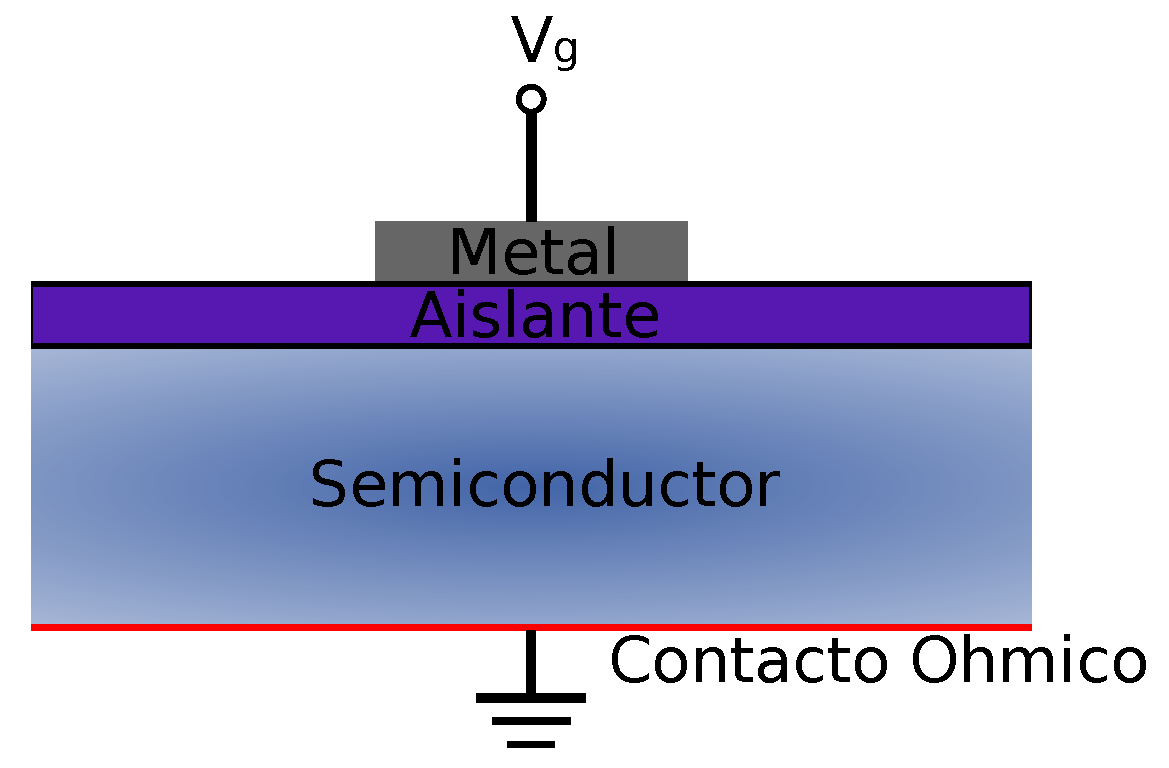
\includegraphics[scale=.35]{Figs/PixelCrossSection.pdf}
    \caption{\footnotesize{Esquema lateral de un capacitor MOS (píxel).}}
    \label{fig:PixelCrossSection}
\end{figure}
\indent El principio de operación de un CCD se puede dividir en cuatro etapas, que a grandes rasgos son:
\begin{itemize}
    \item Exposición del detector: El tiempo de exposición es variable y depende del tipo de medición que se desee utilizar. Durante la exposición, la radiación incidente interactúa con el detector, generalmente generando pares electrón-hueco. 
    \item Colección: Los electrones son luego arrastrados por el campo eléctrico del detector presente en su volumen hacia los pozos de potencial de los píxeles donde son colectados.
    \item Transferencia: Dado que la medición de los píxeles se realiza de forma secuencial, la carga en cada uno de ellos debe ser transferida de un píxel a otro.
    \item Medición de la carga: A medida que se desplaza la carga, esta es llevada hacia el nodo de sensado donde finalmente es medida.
\end{itemize}
Los CCD's convencionales son capaces de alcanzar ruidos de lectura del orden de los $2\,e^{-}\si{rms/pix}$, gracias a la técnica de muestreo doblemente correlacionado\cite{Tiffenberg}. Sin embargo, en aplicaciones de bajas energías, el ruido electrónico de lectura presupone una barrera al límite de energías que pueden medirse con estos sensores para mantener la precisión deseada. Por debajo de los $2\,\si{keV}$ la contribución del ruido de lectura a la determinación de estas cantidades puede superar el $30\,\%$, como se esquematiza en la figura \ref{fig:Fano_y_ruido}. La linea punteada representa el ruido constante de lectura presente en estos sensores y la recta representa un valor constante del factor de Fano para todo el rango de energías. Sobre la curva se ven los puntos que representan los valores del factor de Fano que se medirían si se utilizaran estos sensores debido a la suma de contribuciones del ruido sobre un factor de Fano constante de $0.1$.
\begin{figure}[H]
    \centering
        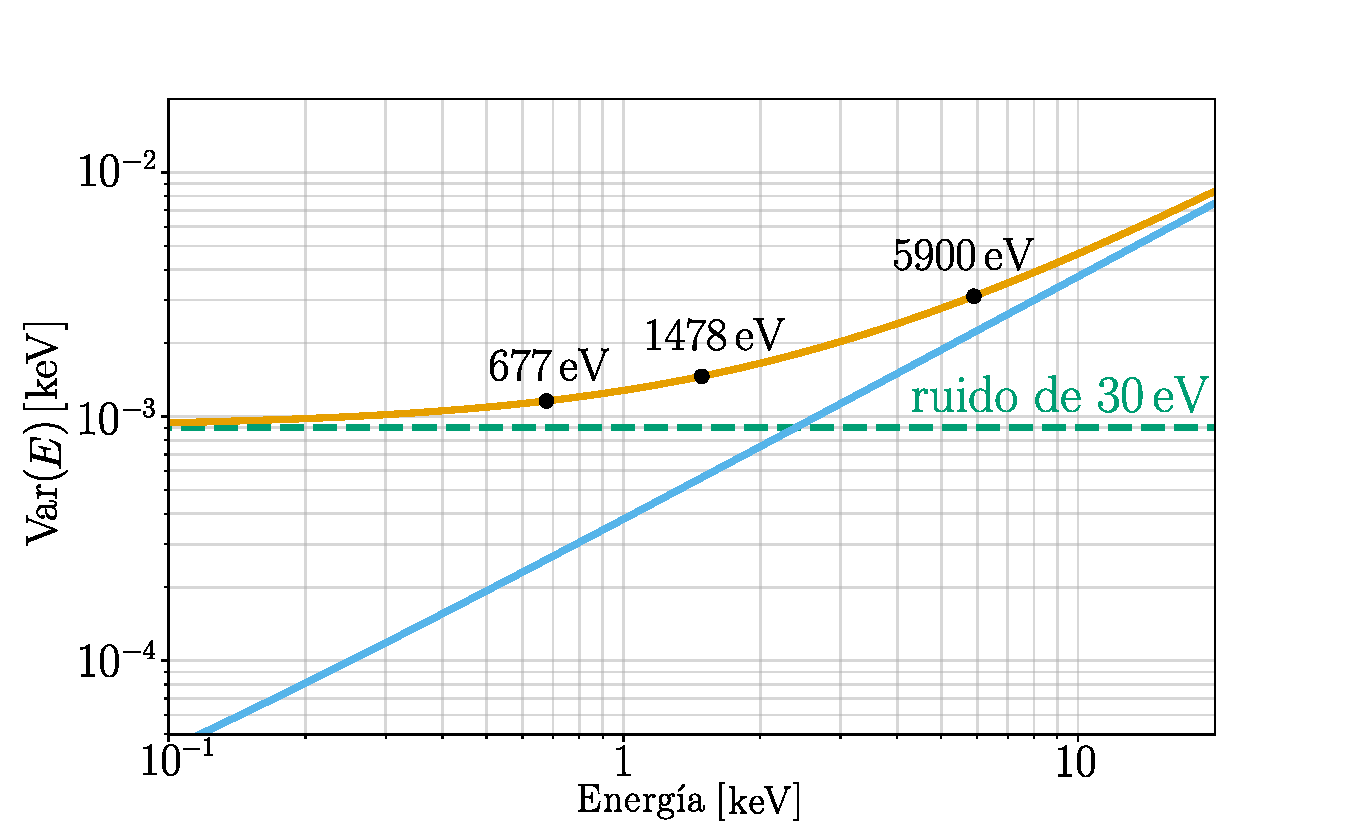
\includegraphics[scale=.5]{Figs/fano_y_ruido.pdf}
    \caption{\footnotesize{Valores queque ta se obtendrían de medir el factor de Fano con un sensor CCD convencional (puntos negros), debido a la contribución del ruido de lectura constante de $30\,\si{eV}$ (linea punteada horizontal). La linea recta continua representa un valor de factor de Fano constante.}}
    \label{fig:Fano_y_ruido}
\end{figure}
Los sensores \textit{Skipper}-CCD's, por otro lado, permiten disminuir el ruido electrónico de lectura a niveles subelectrónicos gracias a que son capaces de medir la carga en los píxeles de forma no destructiva. Esto permite tomar tantas mediciones como sean necesarias de la carga y estimar la carga real a partir de un promedio sobre el número de mediciones tomadas. Esta es la principal razón que motiva este trabajo, donde se realiza un estudio sistemático del factor de Fano a bajas energías, entre $1486\,\si{eV}$ (rayos X del Al) y $677\,\si{eV}$ (rayos X del flúor).\\

%%%%%%%%%%%%%%%%%%%%%%%%%%%%%%%%%%%%%%%%%%%%%%%%%%%%%%%%%%%%%%%%%%
%%%%%%%%%%%%%%%%%%%%%%%%%%%%%%%%%%%%%%%%%%%%%%%%%%%%%%%%%%%%%%%%%%
\subsection{Eficiencia de colección de carga y colección parcial de carga}
\noindent La Eficiencia de Colección de Carga o CCE (\textit{Charge Collection Efficiency}, por sus siglas en inglés) se define como la fracción del total de carga producida durante un evento de ionización que llega a la superficie del píxel del CCD y puede ser finalmente colectada durante el proceso de lectura. Para sensores del tipo \textit{fully depleted} CCD, a los que se les aplican grandes potenciales, la CCE es aproximadamente del $100\,\%$, es decir, toda la carga producida por ionización en el volumen del sensor logra ser colectada y medida. Sin embargo, existen casos donde la eficiencia no alcanza el $100\,\%$ y esto es debido al fenómeno de Colección Parcial de Carga o PCC (\textit{Partial Charge Collection}, por sus siglas en inglés)\cite{PCC-CCE}. Este es un efecto que se debe a que en la región de los primeros micrones cercanos a la superficie existe una probabilidad no nula de que la carga generada por ionización sufra recombinación, es decir, que vuelva a enlazarse a un átomo en vez de ser colectada por el píxel del sensor. Este efecto produce una disminución en el número de cargas que finalmente son llevadas a la superficie del sensor. En el esquema de la figura \ref{fig:PCC} puede verse una vista en corte lateral de un CCD, donde debido al ángulo $\theta$ de incidencia de los rayos $X$ de la fuente, estos fotones generan cargas por ionización en la región donde hay recombinación. Una fracción de las cargas generadas $q_{i}$ logran ser colectadas, dependiendo de la profundidad del sensor donde se produjo la interacción. También se muestra que si la interacción se da fuera de esta región, toda la carga generada por ionización es colectada y $q_{i} = q_{f}$ y la eficiencia es máxima.
\begin{figure}%[H]
%Como reproducir este gráfico: correr el script NivelesOcupacionCarga.py ubicado en /Escritorio/Tesis2021/Figs/pys_para_plots y buscar la imagen en /home/igna/Escritorio/Tesis2021/Figs/
    \centering
        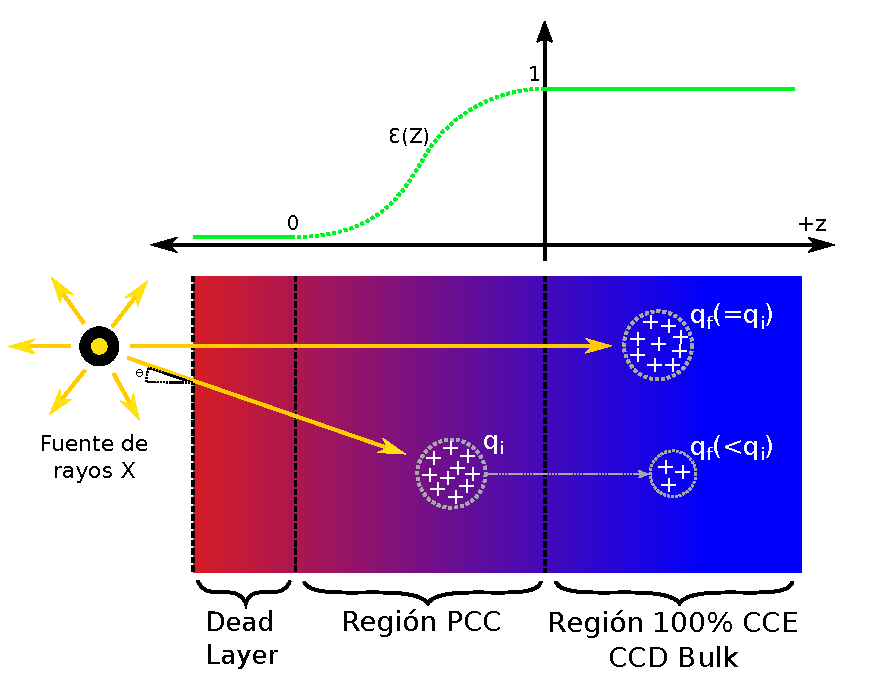
\includegraphics[scale=.8]{Figs/PCC.pdf}
    \caption{\footnotesize{Esquema de un CCD con una fuente de rayos $X$. Los fotones penetran en el sensor produciendo una nube de cargas $q_{i}$, de las cuales solo una fracción logra ser colectada. Esta aumentan monótonamente dependiendo de la profundidad de penetración.}}
    \label{fig:PCC}
\end{figure}
La colección parcial de carga es un problema propio de los sensores y de su fabricación. Sin embargo, existen procesos de fabricación que pueden realizarse sobre la superficie trasera de estos para reducir su efecto, como por ejemplo, los procesos utilizados en la fabricación de CCDs para toma de imágenes astronómicas. %Además, mientras más delgado sea el detector, en general menor es el efecto.

El efecto que provoca la colección parcial de carga en las mediciones es el de agregar eventos con menor cantidad de carga de la que deberían, generando así colas a la izquierda de los picos de interés en los espectros y, por ende, agregando otro sesgo a la determinación de magnitudes dependientes del valor medio de los picos, como el factor de Fano.

%Por otro lado, la profundidad de la interacción depende del ángulo de incidencia y su distribución de probabilidad se puede escribir como
%\begin{equation*}
%    f_{Z}(z) = \frac{\cos{(\theta)}}{\lambda}e^{-z\frac{\cos{(\theta)}}{\lambda}}
%\end{equation*}
%donde $\lambda$ es la longitud de atenuación del fotón y depende de su longitud de onda. $\varepsilon(z)$ es la función \textit{eficiencia de colección de carga}
%\textcolor{red}{Reformulo lo anterior sin la dependencia con $\theta$}:

La física de los fenómenos antes mencionados puede comenzar a modelarse estudiando la distancia que recorren los fotones dentro del sensor hasta interactuar. Esta es una variable aleatoria de distribución exponencial, que viene dada por
\begin{equation*}
    f_{Z}(z) = \frac{1}{\tau_{X}}\exp(-\frac{z}{\tau_{X}})
\end{equation*}
donde $\tau_{X}$ es la longitud de atenuación, que es la distancia promedio para la cual de una población de fotones incidentes solo quede una fracción de $1/e$ de todos ellos. Este es un valor tabulado tanto para la energía de los fotones como para el material. Realizaciones de la variable aleatoria de esta distribución son las diferentes distancias que puede alcanzar un fotón que penetra en el sensor hasta generar cargas por ionización.

También existe una función para caracterizar la eficiencia de la colección de carga, tal que para una dada distancia de penetración $z$, indica qué porcentaje de la carga logra ser colectada y viene dada por
\begin{equation*}
    E_{ff}(z) = 1 - e^{-\frac{z}{\tau_{\scaleto{CEE}{2pt}}}}
\end{equation*}
donde $\tau_{CCE} = 1 - \tau_{X}$, es decir, es la distancia para la cual (estoy quemado, no sé como era esto. ver mañana). 

Si se inyecta la variable aleatoria $z$ que viene de realizaciones de la distribución $f_{Z}$ dentro de la función $E_{ff}(z)$, mediante un cambio de variables la nueva distribución puede reescribirse como
\begin{equation*}
    f_{E_{ff}}(z) = \beta (1 - \varepsilon)^{\beta - 1}
\end{equation*}
donde el parámetro $\beta = \frac{\tau_{\scaleto{CCE}{3pt}}}{\tau_{X}}$. Esta es la distribución de probabilidad de colectar la carga producida por un fotón de una dada energía.

Sin embargo, para terminar de modelar todos los efectos que contribuyen a la dispersión de la carga generada por la interacción de fotones con el material, hay que considerar que, omitiendo todos los efectos anteriores, para una dada energía no siempre se producirán la misma cantidad de ionizaciones. Este efecto es descripto por el factor de Fano. Dado que cada proceso de ionización puede considerarse como un experimento de Bernoulli, una sucesión de interacciones puede pensarse como un fenómeno binomal. En el límite, donde la probabilidad de ionización es baja y la cantidad de veces que puede haber interacciones es muy alta, el proceso se vuelve Poissoniano. Cuando la esperanza de dicha distribución es alta (mayor a 100 en los casos de interes en esta tesis), el límite gaussiano dado por el teorema central del límite se cumple en excelente aproximación. De aquí viene que para agregar esta última contribución al modelado del fenómeno es necesario realizar la convolución de ambas distribuciones. De hacer este cálculo se obtiene la siguiente expresión
\begin{equation*}
    f_{Q_{f}}(q_{f}) = 
    \int\limits_{0}^{1}
    \frac{\beta}{\sqrt{2\pi \sigma^{2}}\varepsilon}
    \exp[%
    -\frac{(q_{f}-\varepsilon\mu)^{2}}{2\sigma^{2}\varepsilon^{2}}
    ](1-\varepsilon)^{\beta - 1}
    d\varepsilon
\end{equation*}
para la distribución teórica de carga debido a los efectos del factor de Fano y la colección parcial de carga actuando conjuntamente.

%\indent Si el detector fuera perfecto, el factor de Fano existiría igual. Este no es un problema del detector, viene del proceso de interacción en sí mismo que a la larga es un fenómeno binomial. Sin embargo, lo que sí es un problema del detector es la PCC. Un fotón interactuando con materia es un experimento Bernoulli, una serie de procesos de interacción es un fenómeno binomial y, en consecuencia, en el límite de probabilidades pequeñas y gran número de repeticiones, de Poisson. Por lo tanto, cuán lejos llega es una variable aleatoria con distribución exponencia (La distancia entre dos eventos de poisson es exponencial). Si uno quiere saber cuál es la probabilidad de que un fotón penetre una dada distancia, hay que hacer
%\begin{equation*}
%    e^{-\frac{d}{\tau}}
%\end{equation*}
%con $\tau$ es la attenuation length. La eficiencia de colección de carga viene dada por 
%\begin{equation*}
%    E_{ff}(z) = 1 - e^{-\frac{z}{\tau_{\scaleto{CEE}{2pt}}}}
%\end{equation*}
%que quiere decir que si la interacción se realizó para un dado $z_{0}$, entonces por ejemplo el $70\%$ de la carga logró ser colectada. Para $Z_{0}$ muy chico, la eficiencia es muy chica, para $z_{0}$ creciente, la eficiencia es creciente.

%Dada la variable aleatoria: Longitud penetrada hasta interactuar, tiene una distribución exponencial. Dada una energía fija, la longitud que recorre hasta interactuar no es siempre la misma, hay una aleatoria inherente. La distribución de probabilidades de este experimento es exponencial. Si por ejemplo la probabilidad de interactuar en los primeros $3\,\si{\mu m}$ es del $50\%$, la probabilidad de interactuar recién luego de recorridos $80\,\si{\mu m}$ es $10^{-14}$. Esta variable aleatoria se inyecta dentro de la función $E_{ff}(z)$: Función a la que le digo hasta donde llegó la partícula antes de interactuar y devuelve con qué eficiencia colectó la carga.

%Se tiene la energía del fotón, se genera un evento aleatorio con distribución exponencial $z_{0}$ que dice qué distancia penetró el fotón antes de interactuar. Esa realización se usa como argumento de $E_{ff}(z) \longrightarrow E_{ff}(z_{0})$. Ese cambio de variables da como resultado 
%\begin{equation*}
%    f_{E_{ff}}(z) = \beta (1 - \varepsilon)^{\beta - 1}
%\end{equation*}
%donde $\beta = \frac{\tau_{\scaleto{CCE}{3pt}}}{\tau_{\scaleto{X}{3pt}}}$. La probabilidad de recuperar la carga de un fotón de una dada energía sigue esa distribución.

%Todavía no entró el Fano. A esto hay que agregarle que además de haber una distribución de carga para la profundidad, además de haber una función que dice cuánta carga se logra colectar con esa profundidad, hay otra variable aleatoria que es cuántos electrones se ionizan cuando se interactúa, que viene de una poissoniana, pero en el límite se puede pensar como una gaussiana. Entonces, a la función anterior hay que convolucionarla con una gaussiana. El efecto de convolucionar una gaussiana con esta distribución es añadirle una cola del lado izquierdo a la gaussiana. De hacer esa convolución se obtiene
%\begin{equation*}
%     f_{Q_{f}}(q_{f}) = 
%     \int\limits_{0}^{1}
%     \frac{\beta}{\sqrt{2\pi \sigma^{2}}\varepsilon}
%     \exp[%
%     -\frac{(q_{f}-\varepsilon\mu)^{2}}{2\sigma^{2}\varepsilon^{2}}
%     ](1-\varepsilon)^{\beta - 1}
%     d\varepsilon
% \end{equation*}
%La cola que aparece a la izquierda es culpa de la PCC, debido a que hay eventos con menor carga generada debido a este fenómeno de recombinación para los eventos que suceden en los primeros micrones del detector. Del lado derecho no hay nada porque no hay un fenómeno que genere más carga de la que el proceso de ionización puede generar.
%%%%%%%%%%%%%%%%%%%%%%%%%%%%%%%%%%%%%%%%%%%%%%%%%%%%%%%%%%%%%%%%%%
%%%%%%%%%%%%%%%%%%%%%%%%%%%%%%%%%%%%%%%%%%%%%%%%%%%%%%%%%%%%%%%%%%
\section{Antecedentes}

\noindent En trabajos previos se han estudiado las ventajas de la utilización de la novedosa tecnología \textit{Skipper} en los CCDs, para lograr medir con precisión subelectrónica en regímenes de energía donde los sensores CCD convencionales más precisos sólo podrían alcanzar resoluciones del orden de los $2$ electrones. Por primera vez fue usada para poder medir el factor de Fano y la energía de creación electrón-hueco en el Silicio a una energía de $5.9\,\si{keV}$ a $123\,\si{K}$\cite{Rodrigues}.\\
\indent Para lograr esto, se implementó un método de calibración absoluta que determinó la relación entre el número de electrones en cada píxel y la lectura del valor en ADUs (\textit{Analog Digital Unit} o Unidades analógico-digitales). El procedimiento para la calibración consistió en la utilización de un LED %instalado en el \textit{dewar}, 
que emitía fotones en $405\,\si{nm}$ de longitud de onda, para poblar los píxeles del sensor. Así, lograron poblar los píxeles con un amplio rango de cargas realizando un barrido en el tiempo de exposición del sensor a la luz LED. La medición de carga se realizó tomando $300$ lecturas por cada píxel, gracias a la tecnología \textit{Skipper} que permite realizar múltiples muestreos de forma no destructiva, que luego fueron promediadas logrando reducir el ruido de lectura en un factor $\sqrt{300}$. Como resultado, se obtuvieron distribuciones de carga Gaussianas en los posibles niveles de ocupación de carga, con suficiente resolución para cada nivel, haciendo posible distinguir perfectamente entre picos consecutivos, como se puede ver en la figura \ref{fig:Calibracion}. De esta forma, mediante un ajuste gaussiano se pudo establecer el valor medio en ADUs para cada uno de estos picos, estableciendo como valor de carga el número de pico correspondiente. Así es que se obtuvo una relación $1$ a $1$ entre cantidad de carga por píxel y ADUs. Cabe destacar que para comenzar a numerar los picos, primero es necesario establecer el valor de $0$ carga, es decir, píxel vacío, lo cual no corresponde, a priori, a un valor nulo en ADUs. Para ello, las imágenes tomadas con \textit{Skipper} cuentan con una región denominada \textit{overscan} que se utiliza para calcular la linea de base y poder substraerla luego a la carga de cada píxel, logrando así que la media de los píxeles vacíos quede en cero ADUs.
\begin{figure}[H]
%Como reproducir este gráfico: correr el script NivelesOcupacionCarga.py ubicado en /Escritorio/Tesis2021/Figs/pys_para_plots y buscar la imagen en /home/igna/Escritorio/Tesis2021/Figs/
    \centering
        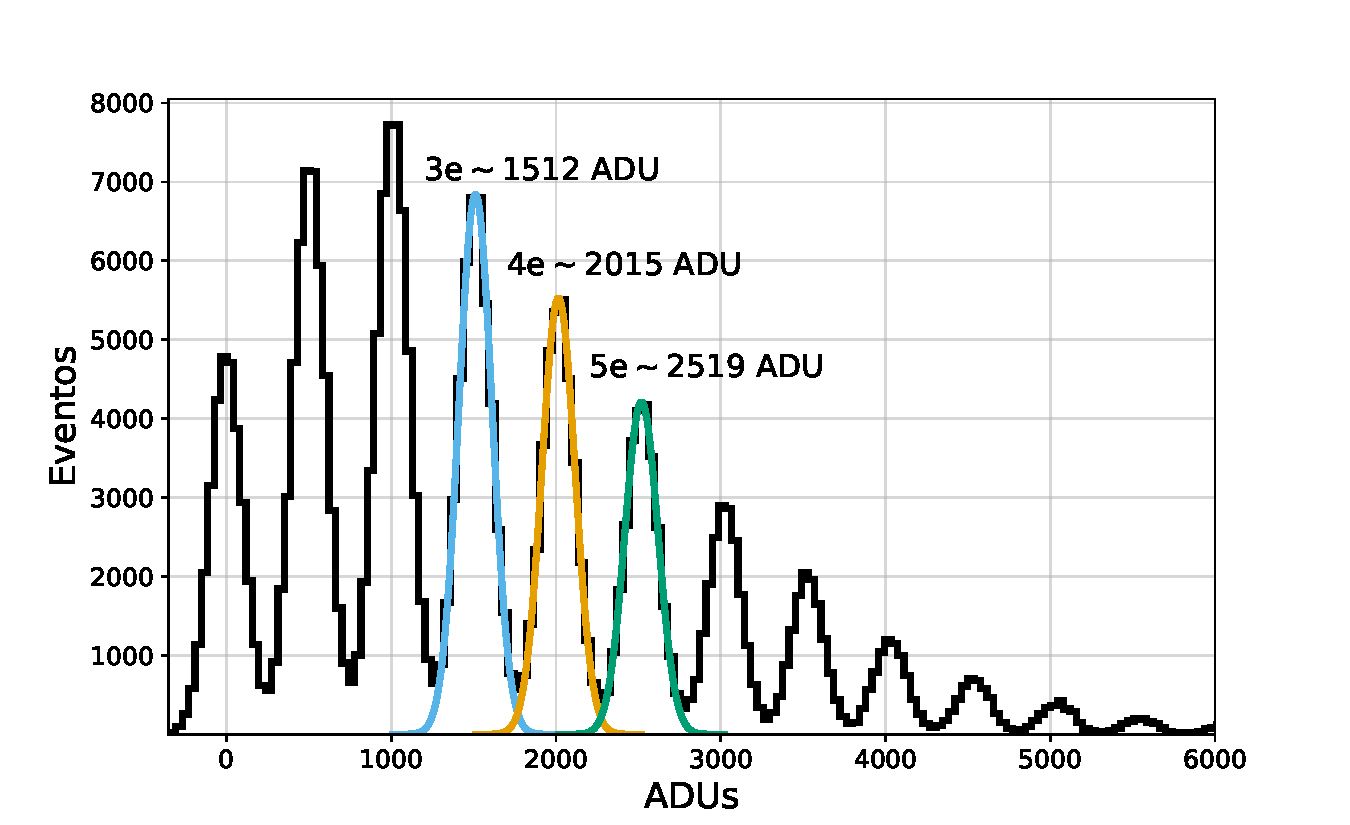
\includegraphics[scale=.5]{Figs/ajuste_gaussiano_calibracion.pdf}
    \caption{\footnotesize{Histograma de los datos obtenidos al iluminar el CCD con LED, correspondiente a una región con poca ocupación, donde los picos de los ajustes entre electrones se distinguen a la perfección.}}
    \label{fig:Calibracion}
\end{figure}
Gracias a esto, por primera vez se midieron el factor de Fano $F$ de forma absoluta y la energía de creación electrón-hueco $\varepsilon_{\eh}$ utilizando esta tecnología. Esto se realizó midiendo rayos $X$ de $5.9\,\si{\mbox{keV}}$ emitidos por una fuente de $\prescript{55}{}{\mbox{Fe}}$. Más precisamente, rayos $X_{K}$, cuyas energías son los de la tabla \ref{tab:EnergiasXk}.
\begin{table}[h]
\centering
\begin{tabular}{@{}ccc@{}}
\toprule
$X_{K}$         &   Energía [keV]   &   Intensidad relativa \\ \hline \hline
$\alpha_{2}$    &   $5887.6$        &   $8.5 (4)$           \\
$\alpha_{1}$    &   $5898.8$        &   $16.9 (8)$          \\
$\beta_{3}$     &   $6490.4$        &   $4.1 (11)$          \\ \bottomrule
\end{tabular}
\caption{\footnotesize{Energías e intensidades relativas de los fotones X emitidos tras el decaimiento de $\prescript{55}{}{\mbox{Fe}}$}}
\label{tab:EnergiasXk}
\end{table}
Sobre los resultados de las mediciones realizadas para estos rayos $X$, se realizó un ajuste de los picos del espectro utilizando la verosimilitud, cuya expresión es la de la ecuación \eqref{ec:verosimilitud}, que surge de la convolución de dos distribuciones exponenciales y una distribución gaussiana
{\small
\begin{align}
    \Lagr(e|\mu_{1},
            \mu_{2},
            \sigma_{1},
            \lambda_{1},
            \lambda_{2},
            \eta_{1} = \eta_{2},
            \eta_{3})
    = &
    \sum\limits_{j=1}^{3} I_{j}
    \left\{
        \eta_{j}\frac{\lambda_{1}}{2}
        \exp
            \left[
                (e-\mu_{j})\lambda_{1} + \frac{\sigma_{j}^{2}\lambda_{1}^{2}}{2}
            \right]
        \mbox{Erfc}
        \left[
            \frac{1}{\sqrt{2}}
            \left(
                \frac{e - \mu_{j}}{\sigma_{j}}
                +\sigma_{j}\lambda_{1}
            \right)
        \right] \right. \nonumber
        \\
        + &
        \left.
        (1-\eta_{j})\frac{\lambda_{2}}{2}
        \exp
            \left[
                 (e - \mu_{j})\lambda_{2}
                 + \frac{\sigma_{j}^{2}\lambda_{2}^{2}}{2}
            \right]
        \mbox{Erfc}
        \left[
            \frac{1}{\sqrt{2}}
            \left(
                \frac{e - \mu_{j}}{\sigma_{j}}
                +\sigma_{j}\lambda_{2}
            \right)
        \right]
    \right\}
        \label{ec:verosimilitud}
\end{align}
}
donde $\mu_{j}$, $\sigma_{j}$ y $I_{j}$ representan el valor medio de carga, la desviación estándar del valor medio de carga y la intensidad relativa del pico $j$-ésimo con energía $E_{j}$, respectivamente. Además, $\lambda_{1}$ y $\lambda_{2}$ son parámetros de la distribuciones exponenciales y $\eta_{j}$ es el peso relativo entre ellas.\\
\indent La figura \ref{fig:AjusteNoBineado} representa el ajuste mediante la verosimilitud de los picos de rayos $X$ para un total de $18085$ eventos. Lo resultados para la medición del factor de Fano, la energía de creación electrón-hueco y demás parámetros relevantes se encuentran en la tabla \ref{tab:ParametrosAjusteNoBineado}.
\begin{figure}%[H]
    \centering
        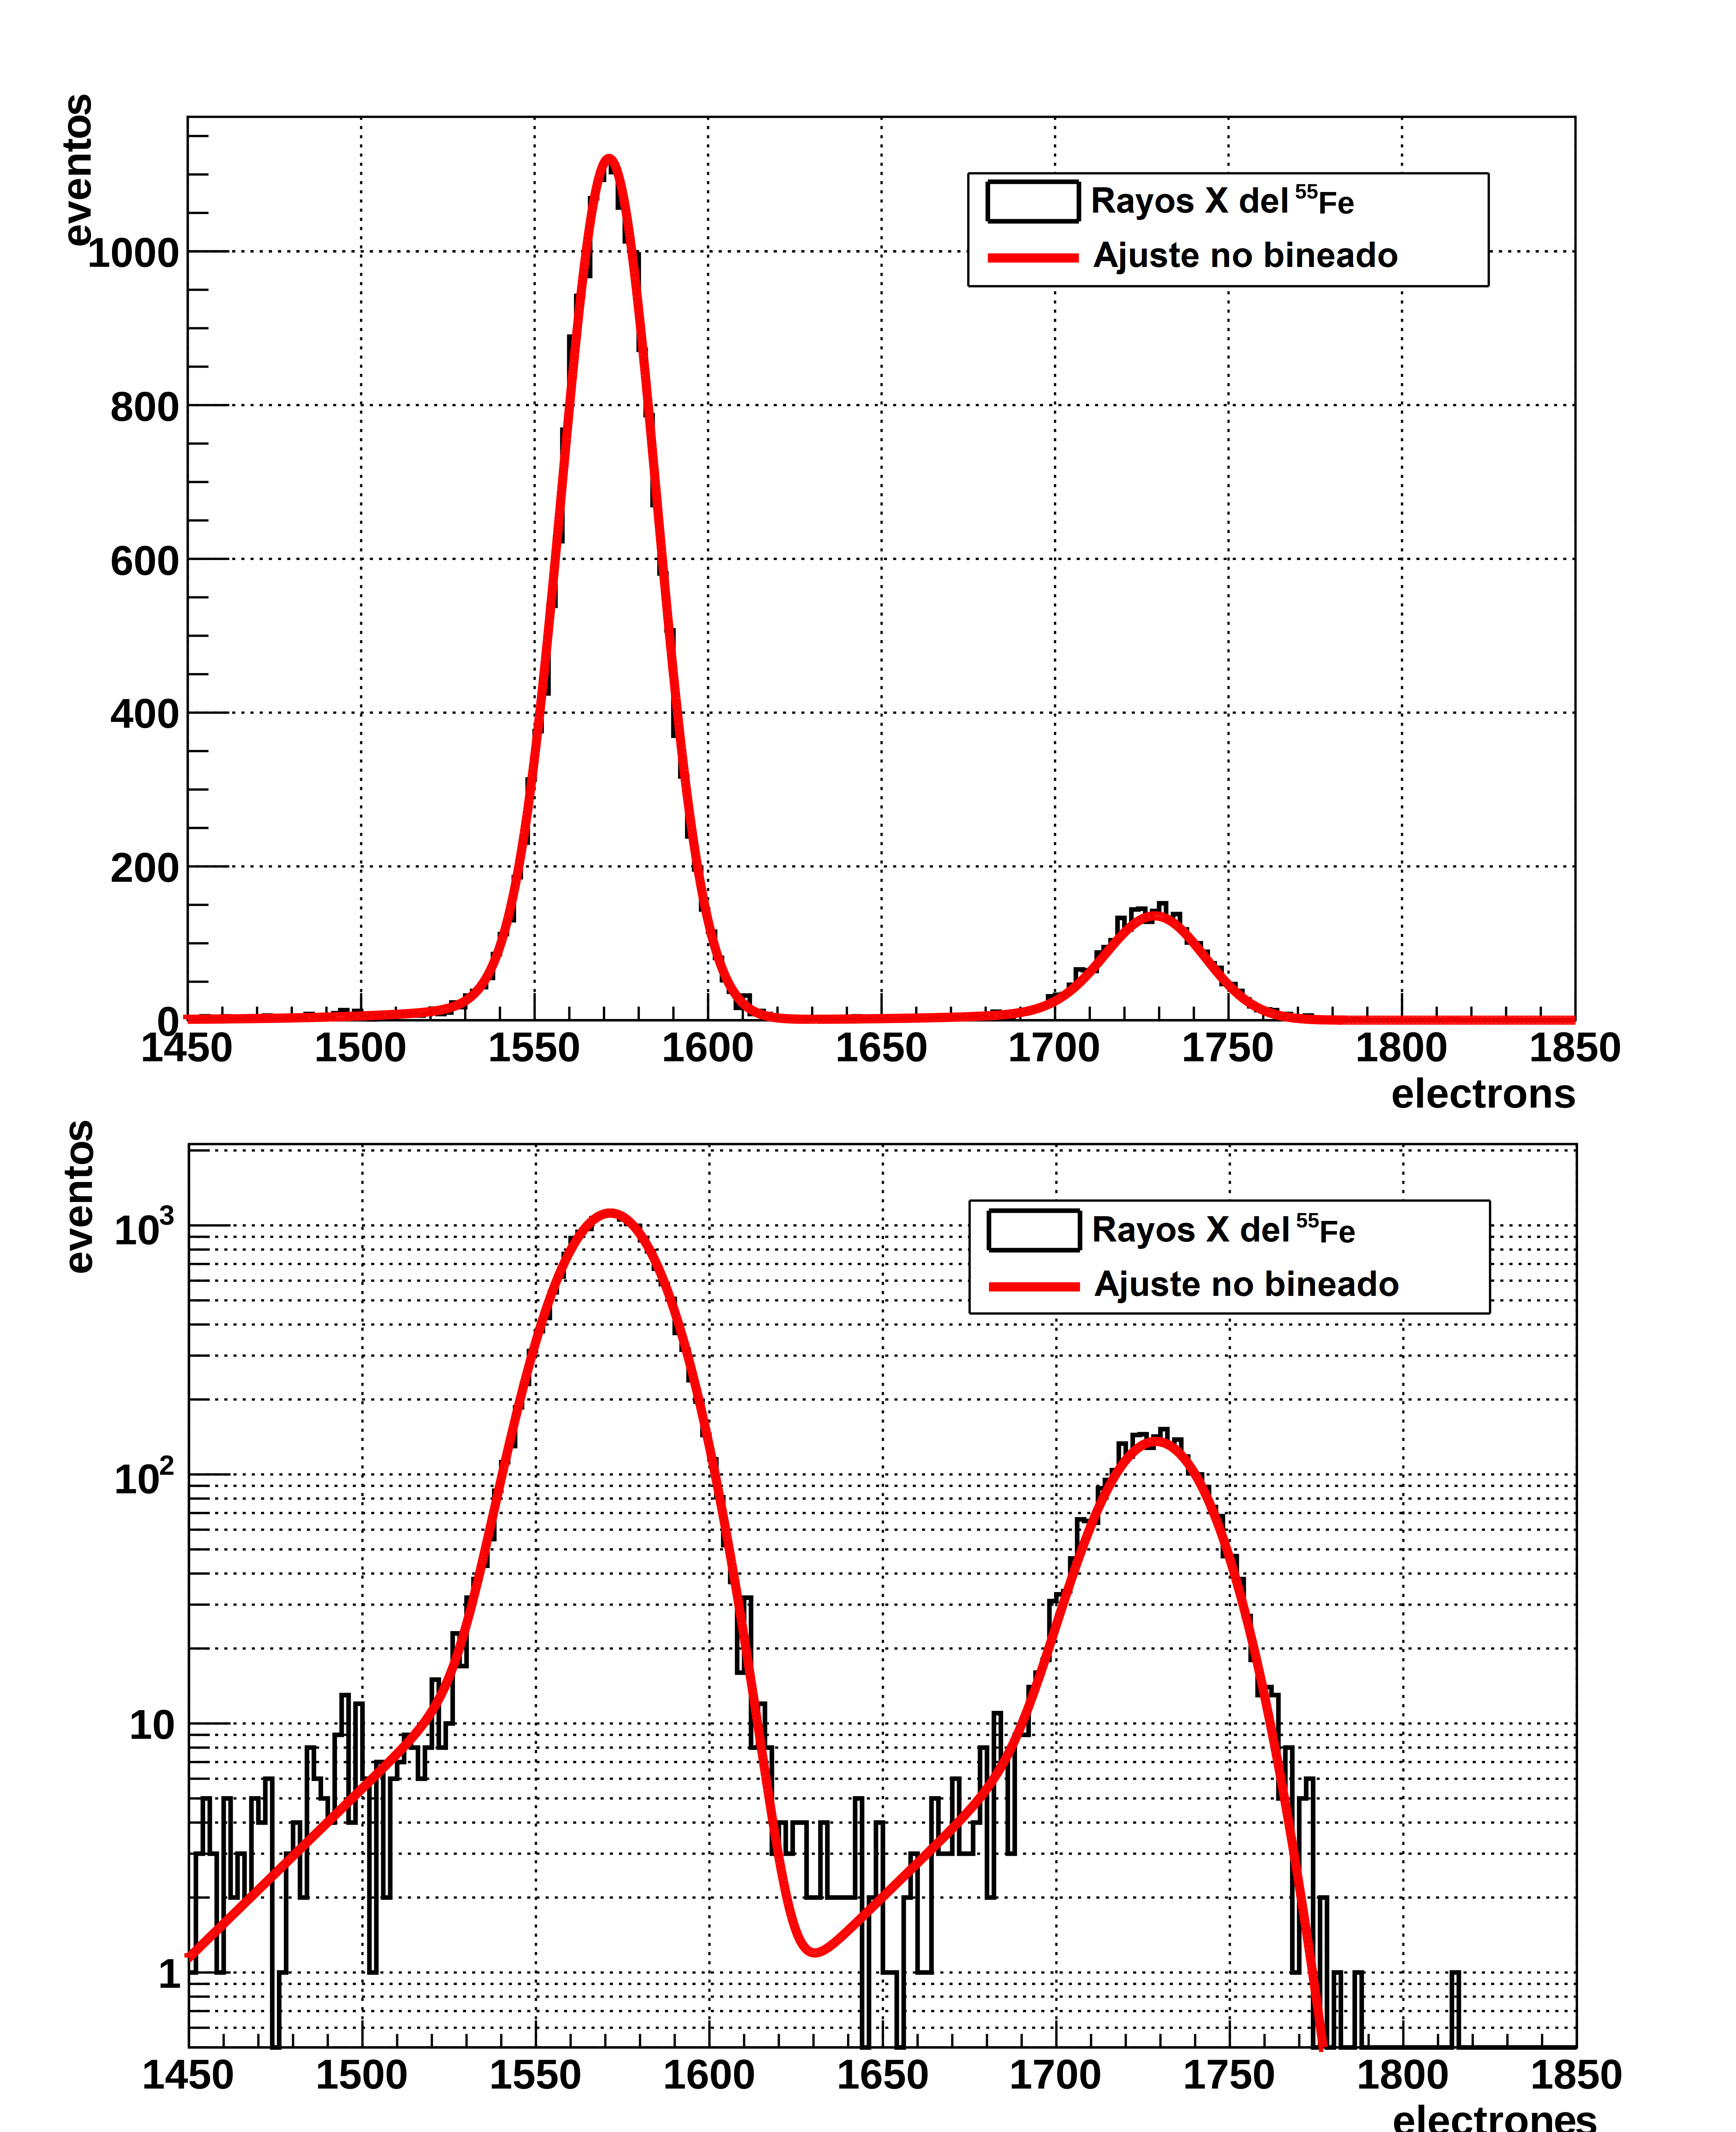
\includegraphics[scale=.15]{Figs/AjusteNoBineado.png}
    \caption{\footnotesize{Ajuste no bineado de los picos de $\prescript{55}{}{\mbox{Fe}}$.}}
    \label{fig:AjusteNoBineado}
\end{figure}
\begin{table}[h]
\centering
\begin{tabular*}{\textwidth}{c @{\extracolsep{\fill}} ccccccccc}%{@{}ccccccccc@{}}
\toprule
$X_{K}$ &
  $\mu\ [e^{-}]$ &
  $\Delta \mu\ [e^{-}]$ &
  $\sigma\ [e^{-}]$ &
  $\Delta \sigma\ [e^{-}]$ &
  $F$ &
  $\Delta F$ &
  $\varepsilon_{\eh}\ [\mbox{eV}/e^{-}]$ &
  $\Delta \varepsilon_{\eh} \ [\mbox{eV}/e^{-}]$ \\ \hline\hline
$\alpha_{2}$ &
  $1570.50$ &
  $0.18$ &
  $13.68$ &
  $0.12$ &
  \multirow{3}{*}{$0.119$} &
  \multirow{3}{*}{$0.002$} &
  \multirow{2}{*}{$3.749$} &
  \multirow{2}{*}{$0.001$} \\
$\alpha_{1}$ & $1573.48$ & $0.18$ & $13.69$ & $0.12$ &  &  &         &         \\
$\beta_{3}$  & $1730.50$ & $0.55$ & $14.36$ & $0.13$ &  &  & $3.751$ & $0.002$ \\ \bottomrule
\end{tabular*}
\caption{tabla}
\label{tab:ParametrosAjusteNoBineado}
\end{table}
Estos constituyen los primeros resultados obtenidos de la utilización de la tecnología \textit{Skipper}-CCD para el cálculo del factor de Fano y de la energía de creación electrón-hueco para una temperatura de $123\,\si{K}$ y se encontraron en buen acuerdo con la bibliografía preexistente~\cite{Ryan, Alig, Kotov}.\\
%Comentarios
\indent Además, se avanzó en las primeras mediciones del factor de Fano y la energía de creación electrón-hueco para energías por debajo de los de $2\,\si{keV}$~\cite{TesisKevin}, más específicamente, para energías de $677\,\si{eV}$ y $1486\,\si{eV}$, que corresponden a los rayos $X$ de fluorescencia del flúor y del aluminio respectivamente. En la tabla \ref{tab:EnergiasFluorescenciaFAl} pueden verse las energías e intensidades relativas para los rayos $X$ de estos elementos. En este caso, utilizando toda la maquinaria desarrollada en el trabajo anterior, realizaron mediciones con una fuente de $\prescript{241}{}{\mbox{Am}}$ que emite partículas alfa con una energía de $\sim 5.6\,\si{MeV}$. A estas partículas luego se las hizo impactar contra una cinta de teflón y una barra de aluminio que por fluorescencia emitían rayos $X$ con las energías antes mencionadas. Cabe destacar que se trató de evitar que las partículas alfa alcanzaran el detector, dado que son partículas muy energéticas y por tanto no son eventos de interés.\\
\indent Uno de los desafíos que surgieron en este otro trabajo fue que solo una fracción de los átomos que son impactados por las partículas alfa se desexcitan emitiendo fotones $X$ en las energías de interés. Es por esto que la tasa de eventos medidos es considerablemente menor en comparación a la que se obtuvo al medir con la fuente de $\prescript{55}{}{\mbox{Fe}}$.
\begin{table}[h]
\centering
\begin{tabular}{@{}cccc@{}}
\toprule
Elemento    &   $X_{K}$         &   Energía [eV]    &   Intensidad relativa \\ \hline \hline
F           &   $\alpha_{1,2}$  &   $676.8$         &   $148$               \\
Al          &   $\alpha_{2}$    &   $1486.3$        &   $50$                \\
Al          &   $\alpha_{1}$    &   $1486.7$        &   $100$               \\
Al          &   $\beta_{1}$     &   $1557.4$        &   $1$                 \\ \bottomrule
\end{tabular}
\caption{\footnotesize{Caption}}
\label{tab:EnergiasFluorescenciaFAl}
\end{table}
Con los datos de estas mediciones se reconstruyeron los espectros para ambos picos y se les realizó un ajuste no bineado, similar al utilizado en los experimentos con $\prescript{55}{}{\mbox{Fe}}$, utilizando la verosimilitud descripta por la expresión \eqref{ec:verosimilitudF-Al}.
\begin{align}
    \Lagr(e|\mu,
            \sigma,
            \lambda_{1},
            \lambda_{2},
            \eta)
    = &
    \eta
    \left\{
        \frac{\lambda_{1}}{2}
        \exp\left[
                (e-\mu)\lambda_{1} + \frac{\sigma^{2}\lambda_{1}^{2}}{2}
            \right]
        \mbox{Erfc}
        \left[
            \frac{1}{\sqrt{2}}
            \left(
                \frac{e - \mu}{\sigma}
                +\sigma\lambda_{1}
            \right)
        \right] \right\} \nonumber
        \\
        + &
        (1-\eta)
        \left\{
        \frac{\lambda_{2}}{2}
        \exp
            \left[
                 (e - \mu)\lambda_{2}
                 + \frac{\sigma^{2}\lambda_{2}^{2}}{2}
            \right]
        \mbox{Erfc}
        \left[
            \frac{1}{\sqrt{2}}
            \left(
                \frac{e - \mu}{\sigma}
                +\sigma\lambda_{2}
            \right)
        \right]
    \right\}
        \label{ec:verosimilitudF-Al}
\end{align}
En este caso, el ajuste resultó mucho más sensible a los cambios en el bineado del histograma, debido a que la tasa de eventos registrados para este experimento fue mucho menor. Los resultados obtenidos en este trabajo a partir de los ajustes de estas mediciones se encuentran en la tabla \ref{tab:ParametrosAjusteNoBineadoF-Al}.\\
\begin{table}[h]
\centering
\begin{tabular*}{\textwidth}{c @{\extracolsep{\fill}} ccccccccc}%{@{}ccccccccc@{}}
\toprule
Elemento&
  $\mu\ [e^{-}]$ &
  $\Delta \mu\ [e^{-}]$ &
  $\sigma\ [e^{-}]$ &
  $\Delta \sigma\ [e^{-}]$ &
  $F$ &
  $\Delta F$ &
  $\varepsilon_{\eh}\ [\mbox{eV}/e^{-}]$ &
  $\Delta \varepsilon_{\eh} \ [\mbox{eV}/e^{-}]$ \\ \hline\hline
  F &   $182.0$ &   $0.8$  &   $7.0$   &   $0.7$   &   $0.27$  &   $0.05$  &   $3.72$ &   $0.02$\\
  Al&   $404.4$ &   $0.4$  &   $8.3$   &   $0.3$   &   $0.17$  &   $0.01$  &   $3.679$ &   $0.004$\\ \bottomrule
\end{tabular*}
\caption{tabla}
\label{tab:ParametrosAjusteNoBineadoF-Al}
\end{table}
\indent Hasta aquí los resultados previos obtenidos con la utilización de esta novedosa tecnología de \textit{Skipper}-CCD para la medición del factor de Fano y la energía de creación electrón hueco. Sin embargo, todavía se pueden mejorar los resultados aumentando la estadística de los eventos para las energías inferiores a $2\,\si{keV}$ caracterizando el fondo presente en las imágenes. Para lograr esto es necesario realizar un tratamiento sobre los datos existentes.
%%%%%%%%%%%%%%%%%%%%%%%%%%%%%%%%%%%%%%%%%%%%%%%%%%%%%%%%%%%%%%%%%%
%%%%%%%%%%%%%%%%%%%%%%%%%%%%%%%%%%%%%%%%%%%%%%%%%%%%%%%%%%%%%%%%%%
\section{Motivación del análisis de imágenes}
%\noindent Este trabajo se centró en la determinación del factor de Fano y de la energía de creación electrón-hueco, para energías por debajo de los $2\,\si{keV}$, utilizando mediciones preexistentes. Más precisamente, para las energías de los rayos $X$ de fluorescencia del aluminio de $1486\,\si{eV}$ y del flúor de $677\,\si{eV}$. Con el fin de que la determinación de estas características esté lo menos sesgada posible debido al fondo presente en las imágenes, fue necesario realizar un análisis profundo de los datos.\\
\noindent El fondo presente en las imágenes consiste principalmente en píxeles cuya carga es producida por fluctuaciones térmicas en la red cristalina del silicio del sensor (corrientes oscuras), por eventos de dispersión producidos por rebotes dentro del dispositivo de medición y que no deseados, o producidos por fotones infrarrojos emitidos desde los materiales que rodean al detector y por eventos muy penetrantes provenientes del exterior, como por ejemplo, muones.

El análisis consistió en estudiar el efecto que produce el fondo de las imágenes sobre los eventos de interés: la aglomeración de píxeles con cargas entre $1$ y $2$ electrones alrededor de los clusters, y la carga extra añadida sobre ellos. En muchos casos resulta que los píxeles con eventos de fondo se aglutinan a los clusters, aumentando su tamaño y su carga, o incluso también haciendo de puente entre dos clusters vecinos. Estos son dos efectos indeseados, primero porque sesga la cantidad de carga real en un evento de interés y segundo porque los algoritmos de clusterizacion podrían ignorarlos al no cumplir con los cortes de calidad impuestos, tanto por forma como por cantidad de carga esperada, disminuyendo así la estadística.

Es entonces necesario utilizar un umbral de detección que ignore estos píxeles con carga menor o igual a $2$ electrones, de forma de evitar el aglutinamiento de píxeles con eventos producto de fondo a los clusters de interés y así aumentar la estadística en el conteo de eventos. Pero también es necesario lograr caracterizar este fondo para corregir el sesgo introducido por el nuevo umbral de detección, el cual, también eliminará píxeles con carga genuina. Es por eso que en este trabajo se propuso un análisis de las imágenes que pueda determinar el umbral más conveniente a utilizar y recuperar la mayor cantidad de estadística posible, además de un método para estimar cuántos eventos genuinos son removidos y cuántos eventos espurios hay que remover de los clusters para mejorar así las incertezas del factor de Fano y la energía de creación electrón-hueco a bajas energías.
%%%%%%%%%%%%%%%%%%%%%%%%%%%%%%%%%%%%%%%%%%%%%%%%%%%%%%%%%%%%%%%%%%
%%%%%%%%%%%%%%%%%%%%%%%%%%%%%%%%%%%%%%%%%%%%%%%%%%%%%%%%%%%%%%%%%%
\section{Organización de la tesis}
Esto lo escribo al final y es un resumen de como está armada la tesis.
%%%%%%%%%%%%%%%%%%%%%%%%%%%%%%%%%%%%%%%%%%%%%%%%%%%%%%%%%%%%%%%%%%
%%%%%%%%%%%%%%%%%%%%%%%%%%%%%%%%%%%%%%%%%%%%%%%%%%%%%%%%%%%%%%%%%%
%%%%%%%%%%%%%%%%%%%%%%%%%%%%%%%%%%%%%%%%%%%%%%%%%%%%%%%%%%%%%%%%%%